\chapter{Writing Matters}
\label{chap:WritingMatters}

\section{Basic mechanics}
\label{sec:BasicMechanics} \index{Grammar}

It is not your advisor's job to fix mechanical errors in your thesis
such as punctuation, dangling or misplaced modifiers, or shifts in
tense and perspective. However, these problems often get in the way
of what students are trying to say and can make a manuscript
unreadable. Most students have serious difficulties with the
mechanics of writing. If you think you don't, ask yourself whether
you understand the difference between ``effect" and ``affect."
Should the period in the previous sentence be placed before or after
the quotation mark? Fortunately, you can get help from the BYU
Writing Center. Visit their web site right now
(\href{http://english.byu.edu/WritingCenter/writingtips.htm}
{\url{http://english.byu.edu/WritingCenter/writingtips.htm}}) and
download a series of their one-page handouts that you think will be
most helpful to you. (Hard Copies of the handouts are also available
at the Writing Center, 1010 JKHB.) You may especially consider
downloading the handouts listed in Table~\ref{table:handouts}.

\begin{table}
    \begin{center}
    \begin{tabular}{lll}
    \hline \hline
    &Paragraph Unity and Coherence &\\
    &Comma Splices and Fused Sentences &\\
    &Punctuating Parenthetical Words or Word Groups &\\
    &Punctuating Quotations &\\
    &The Zen of Pronoun Usage &\\
    &Active vs. Passive Voice &\\
    &Shifts and Perspective Defined &\\
    &Combining Sentences &\\
    &Dangling and Misplaced Modifiers &\\
    \hline \hline
    \end{tabular}
    \end{center}
    \caption{\label{table:handouts} A sampling of handouts available from the Reading Writing Center.}
\end{table}

\emph{Before} submitting drafts of portions of your thesis for
review by your peers and by your advisor, please have the common
courtesy of doing the simple things: Always run your spell checker.
\emph{Always} re-read your document \emph{at least} a day after you
have written it and fix all of the obvious things. Use correct page
layout and formatting, including double spacing so that editors can
insert comments. Near the beginning of the writing process, you may
want to take advantage of one-on-one feedback from a tutor in the
Writing Center, which is a free service. Make a half-hour
appointment to discuss any aspect of the writing process. Be aware
that the tutors will not edit your thesis.

\section{American Institute of Physics Style Manual}
\label{sec:AIPManual} \index{AIP manual}

The American Institute of Physics (AIP) promotes physics research
and education in the US and world wide. Their member societies
include such organizations as the American Physical Society (APS)
and the Society of Physics Students (SPS). To promote uniformity
and clarity of writing throughout the physics community, AIP
publishes a Style Manual \cite{AIP1990} that standardizes the rules
for good physics writing. Most physics journals adhere to the AIP
style manual, and you should become familiar with it as you write
your thesis. Download the style manual from the the American
Institute of Physics web site
(\href{http://www.aip.org/pubservs/style.html}{\url{http://www.aip.org/pubservs/style.html}})
and study the section titled ``Writing the paper" starting on page
6. This is worth more than ten quantum mechanics lectures! (I am
not implying that quantum mechanics is unimportant.) Of course,
there are many other sections in the AIP style manual that would be
good for study. (Note: Astronomy journals follow slightly different
style rules, but for department purposes astronomy students are
permitted to follow AIP style rules.)

\section{References}
\label{sec:References} \index{References}

You will be tempted to delay including references in your thesis
until the end of the writing process. This is a big mistake. Prepare
your list of references as you go, from the very beginning of the
writing process. Otherwise, you may fail to give appropriate credit
when you summarize ideas and results, which is a form of plagiarism.
Do not reference work that you have not read (at least in part
including the introduction and conclusion). Developing your list of
references as you write is much less work in the end.

Students often think that the references are not important and are
careless when transcribing author and journal names. You must
double check each detail of every reference listed. Scientists get
very annoyed when their names are misspelled. Journal editors,
referees, and type setters get very annoyed when misinformation and
incorrect protocol are used in references. Advisors get annoyed
when they have to correct the reference lists in theses because
students are casual about it. The references matter. A list of
various references appears at the end of this document as examples.
The list includes a reference to a journal article
\cite{Peatross2000}, a reference to a page in a book
\cite{Jackson1998}, a reference to multiple pages in a book
\cite{Born1980}, a reference to an individual author contribution
to an edited volume \cite{Peatross1996}, a reference to a
conference proceeding \cite{Peatross1999}, a reference to a work
that is not yet published \cite{Ware}, a reference to a
dissertation \cite{Peatross1993}, a reference to a web page
\cite{intel}, and a reference to a private communication
\cite{Peatross}. The AIP style manual includes examples of other
types of references. It also has a complete listing of
abbreviations for journal titles (see Style Manual Appendix G).

Reference numbers should appear in square brackets throughout the
text in numerical order (as shown in the previous paragraph). The
same reference number may appear more than once in the text, but
undue repetition should be avoided. You may place your reference
list at the end of the entire thesis or at the end of each chapter
when there are many chapters (some duplication of references may
result).

\section{Equations}
\label{sec:Equations} \index{Equations}

Punctuate equations appropriate to the sentence that contains them
\cite{AIP1990}. (You get a brownie point if a sentence structure
requires a question mark immediately following an equation, but
this rarely occurs.) Let entire equations function as a noun (or
the restatement of a noun) in a sentence, although it is
permissible to allow an equal sign to function as a verb (less
desirable). All significant equations should be offset to a line of
their own and given a reference number. Small and less important
equations can be embedded within the text unless they require line
numbers for later reference. If a thesis contains many chapters and
many equations, the equations in chapter 1 should be indexed as
(1.1), (1.2), etc., and the equations in chapter 2 indexed as
(2.1), (2.2), etc. The example below, extracted from the middle of
an article, shows a variety of equation usage.

We use a time expectation integral (proposed by Smith in 1970
\cite{Smith1970}) to specify the arrival of the pulse:
\begin{equation}
  {\left< t \right>}_{ {\bf r} } \equiv
  \int^{\infty}_{-\infty}{t \rho \left( {\bf r}, t \right) \textrm{
  d}t}
  \label{eq:arrival} ,
\end{equation}
where $\rho \left( {\bf r} , t \right)$ is a normalized temporal
distribution of the Poynting flux at ${\bf r}$:
\begin{equation}
  \rho \left( {\bf r}, t \right)  \equiv \hat{\eta} \cdot
  {\bf S} \left( {\bf r}, t \right)
  \left/ \hat{\eta} \cdot \int^{\infty}_{-\infty}{{\bf S}
  \left( {\bf r}, t \right) \textrm{ d}t} \right.
  \label{eq:timedistribution} .
\end{equation}
The Poynting vector is defined as as usual:
\begin{equation}
  {\bf S} \left( {\bf r},t \right) \equiv {\bf E} \left( {\bf r},t
  \right) \times \frac{{\bf B} \left( {\bf r},t
  \right)}{\mu_0} . \label{eq:poynttime}
\end{equation}
The denominator of (\ref{eq:timedistribution}) may be transformed
immediately via Parseval's theorem
\begin{equation}
  \int^\infty_{-\infty}{ {\bf S} \left( {\bf r},t \right) \textrm{ d}t
  } = \int^\infty_{-\infty}{ {\bf S} \left( {\bf r},\omega \right)
  \textrm{ d}\omega } \label{eq:parseval} ,
\end{equation}
where the frequency representation of the Poynting vector is given
by
\begin{equation}
  {\bf S} \left( {\bf r},\omega \right) \equiv {\bf E} \left( {\bf r},\omega
  \right) \times \frac{{\bf B}^* \left( {\bf r},\omega
  \right)}{\mu_0} . \label{eq:poyntfreq}
\end{equation}

\section{Figures}
\label{sec:Figures} \index{Figures}

Take the time to generate professional-looking artwork for your
thesis. Schematics of experimental setups should be simple, well
organized, and labeled as illustrated in
Fig.~\ref{fig:MirrorDiagram}. Use vector graphics rather than raster
graphics unless the figure is a photograph.  Figure captions should
be concise and descriptive. Write figure captions using a smaller
font (10 point). For graphs, be sure to include appropriate units
and to provide a legend referring to the different curves as in
Fig.~\ref{fig:DelayPlot}. Each figure should be described carefully
within the text of your thesis.

\begin{figure}
    \centerline{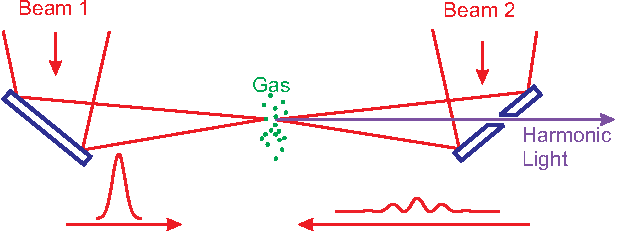
\includegraphics{Graphic1}}
    \caption[Setup for using counter-propagating light]{\label{fig:MirrorDiagram} A mirror with a hole is used to extract high-order harmonics generated in
    counter-propagating laser beams.}
\end{figure}

\begin{figure}
\centerline{\includegraphics[width=5.5in]{figure3}} \caption[Group
delay for broadband pulses]{\label{fig:DelayPlot} (a) Normalized
spectral distribution $\rho$ for the broadband pulse centered on
resonance before (dotted) and after(solid) propagation. (b) Total
delay as a function of $\bar{\omega}$ for the broadband pulse. (c)
Overall pulse transmission as a function of $\bar{\omega}$}
\end{figure}
